% Options for packages loaded elsewhere
\PassOptionsToPackage{unicode}{hyperref}
\PassOptionsToPackage{hyphens}{url}
\PassOptionsToPackage{dvipsnames,svgnames,x11names}{xcolor}
\documentclass[
  11pt,
]{article}
\usepackage{xcolor}
\usepackage[margin=0.85in]{geometry}
\usepackage{amsmath,amssymb}
\setcounter{secnumdepth}{-\maxdimen} % remove section numbering
\usepackage{iftex}
\ifPDFTeX
  \usepackage[T1]{fontenc}
  \usepackage[utf8]{inputenc}
  \usepackage{textcomp} % provide euro and other symbols
\else % if luatex or xetex
  \usepackage{unicode-math} % this also loads fontspec
  \defaultfontfeatures{Scale=MatchLowercase}
  \defaultfontfeatures[\rmfamily]{Ligatures=TeX,Scale=1}
\fi
\usepackage{lmodern}
\ifPDFTeX\else
  % xetex/luatex font selection
\fi
% Use upquote if available, for straight quotes in verbatim environments
\IfFileExists{upquote.sty}{\usepackage{upquote}}{}
\IfFileExists{microtype.sty}{% use microtype if available
  \usepackage[]{microtype}
  \UseMicrotypeSet[protrusion]{basicmath} % disable protrusion for tt fonts
}{}
\makeatletter
\@ifundefined{KOMAClassName}{% if non-KOMA class
  \IfFileExists{parskip.sty}{%
    \usepackage{parskip}
  }{% else
    \setlength{\parindent}{0pt}
    \setlength{\parskip}{6pt plus 2pt minus 1pt}}
}{% if KOMA class
  \KOMAoptions{parskip=half}}
\makeatother
\usepackage{color}
\usepackage{fancyvrb}
\newcommand{\VerbBar}{|}
\newcommand{\VERB}{\Verb[commandchars=\\\{\}]}
\DefineVerbatimEnvironment{Highlighting}{Verbatim}{commandchars=\\\{\}}
% Add ',fontsize=\small' for more characters per line
\newenvironment{Shaded}{}{}
\newcommand{\AlertTok}[1]{\textcolor[rgb]{1.00,0.00,0.00}{\textbf{#1}}}
\newcommand{\AnnotationTok}[1]{\textcolor[rgb]{0.38,0.63,0.69}{\textbf{\textit{#1}}}}
\newcommand{\AttributeTok}[1]{\textcolor[rgb]{0.49,0.56,0.16}{#1}}
\newcommand{\BaseNTok}[1]{\textcolor[rgb]{0.25,0.63,0.44}{#1}}
\newcommand{\BuiltInTok}[1]{\textcolor[rgb]{0.00,0.50,0.00}{#1}}
\newcommand{\CharTok}[1]{\textcolor[rgb]{0.25,0.44,0.63}{#1}}
\newcommand{\CommentTok}[1]{\textcolor[rgb]{0.38,0.63,0.69}{\textit{#1}}}
\newcommand{\CommentVarTok}[1]{\textcolor[rgb]{0.38,0.63,0.69}{\textbf{\textit{#1}}}}
\newcommand{\ConstantTok}[1]{\textcolor[rgb]{0.53,0.00,0.00}{#1}}
\newcommand{\ControlFlowTok}[1]{\textcolor[rgb]{0.00,0.44,0.13}{\textbf{#1}}}
\newcommand{\DataTypeTok}[1]{\textcolor[rgb]{0.56,0.13,0.00}{#1}}
\newcommand{\DecValTok}[1]{\textcolor[rgb]{0.25,0.63,0.44}{#1}}
\newcommand{\DocumentationTok}[1]{\textcolor[rgb]{0.73,0.13,0.13}{\textit{#1}}}
\newcommand{\ErrorTok}[1]{\textcolor[rgb]{1.00,0.00,0.00}{\textbf{#1}}}
\newcommand{\ExtensionTok}[1]{#1}
\newcommand{\FloatTok}[1]{\textcolor[rgb]{0.25,0.63,0.44}{#1}}
\newcommand{\FunctionTok}[1]{\textcolor[rgb]{0.02,0.16,0.49}{#1}}
\newcommand{\ImportTok}[1]{\textcolor[rgb]{0.00,0.50,0.00}{\textbf{#1}}}
\newcommand{\InformationTok}[1]{\textcolor[rgb]{0.38,0.63,0.69}{\textbf{\textit{#1}}}}
\newcommand{\KeywordTok}[1]{\textcolor[rgb]{0.00,0.44,0.13}{\textbf{#1}}}
\newcommand{\NormalTok}[1]{#1}
\newcommand{\OperatorTok}[1]{\textcolor[rgb]{0.40,0.40,0.40}{#1}}
\newcommand{\OtherTok}[1]{\textcolor[rgb]{0.00,0.44,0.13}{#1}}
\newcommand{\PreprocessorTok}[1]{\textcolor[rgb]{0.74,0.48,0.00}{#1}}
\newcommand{\RegionMarkerTok}[1]{#1}
\newcommand{\SpecialCharTok}[1]{\textcolor[rgb]{0.25,0.44,0.63}{#1}}
\newcommand{\SpecialStringTok}[1]{\textcolor[rgb]{0.73,0.40,0.53}{#1}}
\newcommand{\StringTok}[1]{\textcolor[rgb]{0.25,0.44,0.63}{#1}}
\newcommand{\VariableTok}[1]{\textcolor[rgb]{0.10,0.09,0.49}{#1}}
\newcommand{\VerbatimStringTok}[1]{\textcolor[rgb]{0.25,0.44,0.63}{#1}}
\newcommand{\WarningTok}[1]{\textcolor[rgb]{0.38,0.63,0.69}{\textbf{\textit{#1}}}}
\usepackage{longtable,booktabs,array}
\newcounter{none} % for unnumbered tables
\usepackage{calc} % for calculating minipage widths
% Correct order of tables after \paragraph or \subparagraph
\usepackage{etoolbox}
\makeatletter
\patchcmd\longtable{\par}{\if@noskipsec\mbox{}\fi\par}{}{}
\makeatother
% Allow footnotes in longtable head/foot
\IfFileExists{footnotehyper.sty}{\usepackage{footnotehyper}}{\usepackage{footnote}}
\makesavenoteenv{longtable}
\usepackage{graphicx}
\makeatletter
\newsavebox\pandoc@box
\newcommand*\pandocbounded[1]{% scales image to fit in text height/width
  \sbox\pandoc@box{#1}%
  \Gscale@div\@tempa{\textheight}{\dimexpr\ht\pandoc@box+\dp\pandoc@box\relax}%
  \Gscale@div\@tempb{\linewidth}{\wd\pandoc@box}%
  \ifdim\@tempb\p@<\@tempa\p@\let\@tempa\@tempb\fi% select the smaller of both
  \ifdim\@tempa\p@<\p@\scalebox{\@tempa}{\usebox\pandoc@box}%
  \else\usebox{\pandoc@box}%
  \fi%
}
% Set default figure placement to htbp
\def\fps@figure{htbp}
\makeatother
\setlength{\emergencystretch}{3em} % prevent overfull lines
\providecommand{\tightlist}{%
  \setlength{\itemsep}{0pt}\setlength{\parskip}{0pt}}
\usepackage{amsmath,amssymb}
\usepackage{float}
\usepackage{microtype}
\usepackage{fvextra}
\fvset{breaklines=true}
\usepackage{setspace}
\usepackage{lineno}
\usepackage{etoolbox}
\usepackage{needspace}
\usepackage{xurl}
\AtBeginEnvironment{longtable}{\singlespacing\small}
\AtBeginEnvironment{verbatim}{\singlespacing\small}
\setlength{\emergencystretch}{3em}
\floatplacement{figure}{H}
\DeclareUnicodeCharacter{2212}{\ensuremath{-}}
\DeclareUnicodeCharacter{2264}{\ensuremath{\leq}}
\DeclareUnicodeCharacter{2265}{\ensuremath{\geq}}
\DeclareUnicodeCharacter{2260}{\ensuremath{\ne}}
\DeclareUnicodeCharacter{2208}{\ensuremath{\in}}
\DeclareUnicodeCharacter{221E}{\ensuremath{\infty}}
\DeclareUnicodeCharacter{03B4}{\ensuremath{\delta}}
\DeclareUnicodeCharacter{03BB}{\ensuremath{\lambda}}
\DeclareUnicodeCharacter{03C4}{\ensuremath{\tau}}
\DeclareUnicodeCharacter{03BA}{\ensuremath{\kappa}}
\DeclareUnicodeCharacter{03B3}{\ensuremath{\gamma}}
\DeclareUnicodeCharacter{03B5}{\ensuremath{\varepsilon}}
\DeclareUnicodeCharacter{03C6}{\ensuremath{\phi}}
\DeclareUnicodeCharacter{2124}{\ensuremath{\mathbb Z}}
\DeclareUnicodeCharacter{1D63}{\ensuremath{{}_r}}
\DeclareUnicodeCharacter{2080}{\ensuremath{{}_0}}
\DeclareUnicodeCharacter{208A}{\ensuremath{{}_+}}
\DeclareUnicodeCharacter{208B}{\ensuremath{{}_-}}
\DeclareUnicodeCharacter{207B}{\ensuremath{{}^{-}}}
\DeclareUnicodeCharacter{00B9}{\ensuremath{{}^{1}}}
\DeclareUnicodeCharacter{00B2}{\ensuremath{{}^{2}}}
\DeclareUnicodeCharacter{2074}{\ensuremath{{}^{4}}}
\DeclareUnicodeCharacter{2075}{\ensuremath{{}^{5}}}
\DeclareUnicodeCharacter{2076}{\ensuremath{{}^{6}}}
\DeclareUnicodeCharacter{2192}{\ensuremath{\rightarrow}}
\DeclareUnicodeCharacter{0108}{\ensuremath{\widehat C}}
\DeclareUnicodeCharacter{00C2}{\ensuremath{\widehat A}}

\AtBeginDocument{\setstretch{1.12}}
\usepackage{bookmark}
\IfFileExists{xurl.sty}{\usepackage{xurl}}{} % add URL line breaks if available
\urlstyle{same}
% fallback for those not using the hyperref driver hyperxmp:
\makeatletter
\@ifundefined{xmpquote}{\newcommand{\xmpquote}[1]{#1}}{}
\makeatother
\hypersetup{
  colorlinks=true,
  linkcolor={Maroon},
  filecolor={Maroon},
  citecolor={Blue},
  urlcolor={blue},
  pdfcreator={LaTeX via pandoc}}

\author{}
\date{}

\begin{document}

\section{Additional file 4: Track
portability}\label{additional-file-4-track-portability}

This supplement concerns the same 84 sites and seven genes under a
second AlphaGenome contact track. It is not a new cohort or independent
model. The protocol was locally frozen before acquisition, then
native-only predictions were locked before centered evaluation.

Technical transfer: PASS. Operational benchmark: PASS. The operational
threshold was at least 17 additional leaders and gains in at least four
genes, with no lost simple-bound decisions, complete data and no
validation failures. It is not a powered hypothesis test.

\subsection{Gene-level primary results (tie tolerance
1e-6)}\label{gene-level-primary-results-tie-tolerance-1e-6}

{\def\LTcaptype{none} % do not increment counter
\begin{longtable}[]{@{}
  >{\raggedright\arraybackslash}p{(\linewidth - 12\tabcolsep) * \real{0.1300}}
  >{\raggedleft\arraybackslash}p{(\linewidth - 12\tabcolsep) * \real{0.0800}}
  >{\raggedleft\arraybackslash}p{(\linewidth - 12\tabcolsep) * \real{0.1400}}
  >{\raggedleft\arraybackslash}p{(\linewidth - 12\tabcolsep) * \real{0.1800}}
  >{\raggedleft\arraybackslash}p{(\linewidth - 12\tabcolsep) * \real{0.1300}}
  >{\raggedleft\arraybackslash}p{(\linewidth - 12\tabcolsep) * \real{0.1700}}
  >{\raggedleft\arraybackslash}p{(\linewidth - 12\tabcolsep) * \real{0.1700}}@{}}
\toprule\noalign{}
\begin{minipage}[b]{\linewidth}\raggedright
Gene
\end{minipage} & \begin{minipage}[b]{\linewidth}\raggedleft
Sites
\end{minipage} & \begin{minipage}[b]{\linewidth}\raggedleft
Simple leaders
\end{minipage} & \begin{minipage}[b]{\linewidth}\raggedleft
Strengthened leaders
\end{minipage} & \begin{minipage}[b]{\linewidth}\raggedleft
Additional
\end{minipage} & \begin{minipage}[b]{\linewidth}\raggedleft
Native credit
\end{minipage} & \begin{minipage}[b]{\linewidth}\raggedleft
Centered credit
\end{minipage} \\
\midrule\noalign{}
\endhead
\bottomrule\noalign{}
\endlastfoot
\emph{ASS1} & 12 & 3 & 10 & 7 & 0.250000 & 0.083333 \\
\emph{BAP1} & 12 & 0 & 11 & 11 & 0.333333 & 0.750000 \\
\emph{BRCA2} & 12 & 1 & 8 & 7 & 0.305556 & 0.416667 \\
\emph{HFE} & 12 & 0 & 4 & 4 & 0.347222 & 0.375000 \\
\emph{RB1} & 12 & 2 & 2 & 0 & 0.444444 & 0.416667 \\
\emph{SCN5A} & 12 & 0 & 6 & 6 & 0.347222 & 0.416667 \\
\emph{TSC1} & 12 & 1 & 8 & 7 & 0.319444 & 0.333333 \\
\end{longtable}
}

\subsection{Fixed tolerance
sensitivities}\label{fixed-tolerance-sensitivities}

{\def\LTcaptype{none} % do not increment counter
\begin{longtable}[]{@{}
  >{\raggedright\arraybackslash}p{(\linewidth - 10\tabcolsep) * \real{0.1500}}
  >{\raggedleft\arraybackslash}p{(\linewidth - 10\tabcolsep) * \real{0.1700}}
  >{\raggedleft\arraybackslash}p{(\linewidth - 10\tabcolsep) * \real{0.1700}}
  >{\raggedleft\arraybackslash}p{(\linewidth - 10\tabcolsep) * \real{0.1700}}
  >{\raggedleft\arraybackslash}p{(\linewidth - 10\tabcolsep) * \real{0.1700}}
  >{\raggedleft\arraybackslash}p{(\linewidth - 10\tabcolsep) * \real{0.1700}}@{}}
\toprule\noalign{}
\begin{minipage}[b]{\linewidth}\raggedright
Tie tolerance
\end{minipage} & \begin{minipage}[b]{\linewidth}\raggedleft
Simple leaders
\end{minipage} & \begin{minipage}[b]{\linewidth}\raggedleft
Strengthened leaders
\end{minipage} & \begin{minipage}[b]{\linewidth}\raggedleft
Additional
\end{minipage} & \begin{minipage}[b]{\linewidth}\raggedleft
Native ties
\end{minipage} & \begin{minipage}[b]{\linewidth}\raggedleft
Centered ties
\end{minipage} \\
\midrule\noalign{}
\endhead
\bottomrule\noalign{}
\endlastfoot
0.0 & 7 & 50 & 43 & 75 & 0 \\
1e-05 & 7 & 42 & 35 & 75 & 12 \\
1e-06 & 7 & 49 & 42 & 75 & 1 \\
\end{longtable}
}

\subsection{Fixed baseline
comparisons}\label{fixed-baseline-comparisons}

{\def\LTcaptype{none} % do not increment counter
\begin{longtable}[]{@{}
  >{\raggedright\arraybackslash}p{(\linewidth - 6\tabcolsep) * \real{0.3700}}
  >{\raggedleft\arraybackslash}p{(\linewidth - 6\tabcolsep) * \real{0.2100}}
  >{\raggedleft\arraybackslash}p{(\linewidth - 6\tabcolsep) * \real{0.2100}}
  >{\raggedleft\arraybackslash}p{(\linewidth - 6\tabcolsep) * \real{0.2100}}@{}}
\toprule\noalign{}
\begin{minipage}[b]{\linewidth}\raggedright
Score
\end{minipage} & \begin{minipage}[b]{\linewidth}\raggedleft
IMR-90 selected credit
\end{minipage} & \begin{minipage}[b]{\linewidth}\raggedleft
GM12878 selected credit
\end{minipage} & \begin{minipage}[b]{\linewidth}\raggedleft
IMR-90 agreement with centered top set
\end{minipage} \\
\midrule\noalign{}
\endhead
\bottomrule\noalign{}
\endlastfoot
absolute mean change & 0.410714 & 0.315476 & 58/84 \\
centered & 0.398810 & 0.321429 & 84/84 \\
centered rms & 0.517857 & 0.460317 & 36/84 \\
lifetime count absolute change & 0.349206 & 0.434524 & 33/84 \\
max absolute & 0.341270 & 0.357143 & 10/84 \\
maximum persistence absolute change & 0.353175 & 0.327381 & 16/84 \\
native & 0.335317 & 0.359127 & 9/84 \\
native minus absolute mean change & 0.244048 & 0.380952 & 16/84 \\
native plus absolute mean change & 0.410714 & 0.321429 & 64/84 \\
native rms & 0.500000 & 0.444444 & 39/84 \\
total persistence absolute change & 0.464286 & 0.333333 & 21/84 \\
\end{longtable}
}

Deleting one gene leaves 31--42 additional leaders among 72 sites. The
corresponding centered-minus-native credit ranges from +0.004630 to
+0.101852. These are concentration diagnostics, not independent-sample
uncertainty intervals.

\subsection{Provenance, controls and
precision}\label{provenance-controls-and-precision}

Frozen source hashes and timestamps, all acquisition attempts and the
exact per-site selections are retained in the experiment bundle. The two
central SHA256 records are:

\begin{Shaded}
\begin{Highlighting}[]
\NormalTok{Protocol:}
\NormalTok{56c5ae0650a02f05384e1d1cbc19f894d957d155f196a6db5432f9f36e10aa43}
\NormalTok{Native{-}prediction lock:}
\NormalTok{cc6ddc14d531f8e95974dbb69ae1b8dc3b7fdf73ed0f4201279836e1b52cef40}
\end{Highlighting}
\end{Shaded}

Both track channels were selected by exact metadata name. All 252
requests succeeded on their first attempt. Every repeated REF agreed,
every contemporary GM12878 map equaled its historical counterpart, and
every paired IMR-90 REF/ALT map differed from GM12878. All 132,120,576
delivered float32 values per track, including repeated reference arrays,
were exactly bfloat16-representable. Equal outputs at these inputs do
not establish immutable weights or biological measurement precision.

Nine phased-engine controls tested scientific equivalence,
missing/changed locks, changed protocol, nonsaturation and wrong-leader
detection. Twelve summary boundary controls tested the operational
thresholds and incomplete data. The full replay checked 3696 scientific
comparisons; 3696 were exactly equal. The independent per-site audit
reports status PASS and maximum Hausdorff difference 0.

Bounds apply to the stored floating-point diagrams with a practical
1e-12 allowance, not a rigorous arithmetic enclosure. The matching
solver uses zero approximation parameter. Added PH input rounding,
observed grid structure and identical repeated outputs are separately
described; none recovers latent model uncertainty. No runtime advantage,
clinical accuracy improvement or experimental chromatin mechanism is
established. No new clinical testing family was introduced.

The full protocol, machine-readable summary, independent audit, replay
comparison and preserved execution correction accompany this supplement.
Original discovery and replication evidence remains separately reported.

\subsection{Post-result direct path
diagnostics}\label{post-result-direct-path-diagnostics}

After the primary results were known, a separate local protocol
specified direct evaluations of all three nonsaturating comparisons on
the grid lambda = 0, 0.1, 0.25, 0.5, 0.75, 0.9 and 1. The diagnostic
protocol and code were hashed before these additional queries. Selection
was explicitly outcome-dependent and included all exceptions, with no
change to the original cohort, primary endpoint or saved predictions.

\Needspace{9\baselineskip}

{\def\LTcaptype{none} % do not increment counter
\begin{longtable}[]{@{}
  >{\raggedright\arraybackslash}p{(\linewidth - 4\tabcolsep) * \real{0.4800}}
  >{\raggedright\arraybackslash}p{(\linewidth - 4\tabcolsep) * \real{0.2600}}
  >{\raggedleft\arraybackslash}p{(\linewidth - 4\tabcolsep) * \real{0.2600}}@{}}
\toprule\noalign{}
\begin{minipage}[b]{\linewidth}\raggedright
RB1 site (GRCh38), alternate index
\end{minipage} & \begin{minipage}[b]{\linewidth}\raggedright
Sampled behavior
\end{minipage} & \begin{minipage}[b]{\linewidth}\raggedleft
Maximum departure from endpoint chord
\end{minipage} \\
\midrule\noalign{}
\endhead
\bottomrule\noalign{}
\endlastfoot
chr13:48303721:G, 2 & Direction changes on sampled grid & 0.000903 \\
chr13:48307406:G, 1 & Direction changes on sampled grid & 0.00129 \\
chr13:48465370:T, 0 & Flat on sampled grid & 1.08e-16 \\
\end{longtable}
}

Alternate indices are zero-based in the saved alphabetical non-reference
allele order. All 21 direct distances satisfied the two-endpoint
envelopes, and endpoint recomputations agreed within 1e-12. Both simple
and strengthened bounds had already abstained at all three sites at all
fixed tolerances. This is conservative behavior shared by both bounds;
it is not the witness-specific incremental advantage.

\pandocbounded{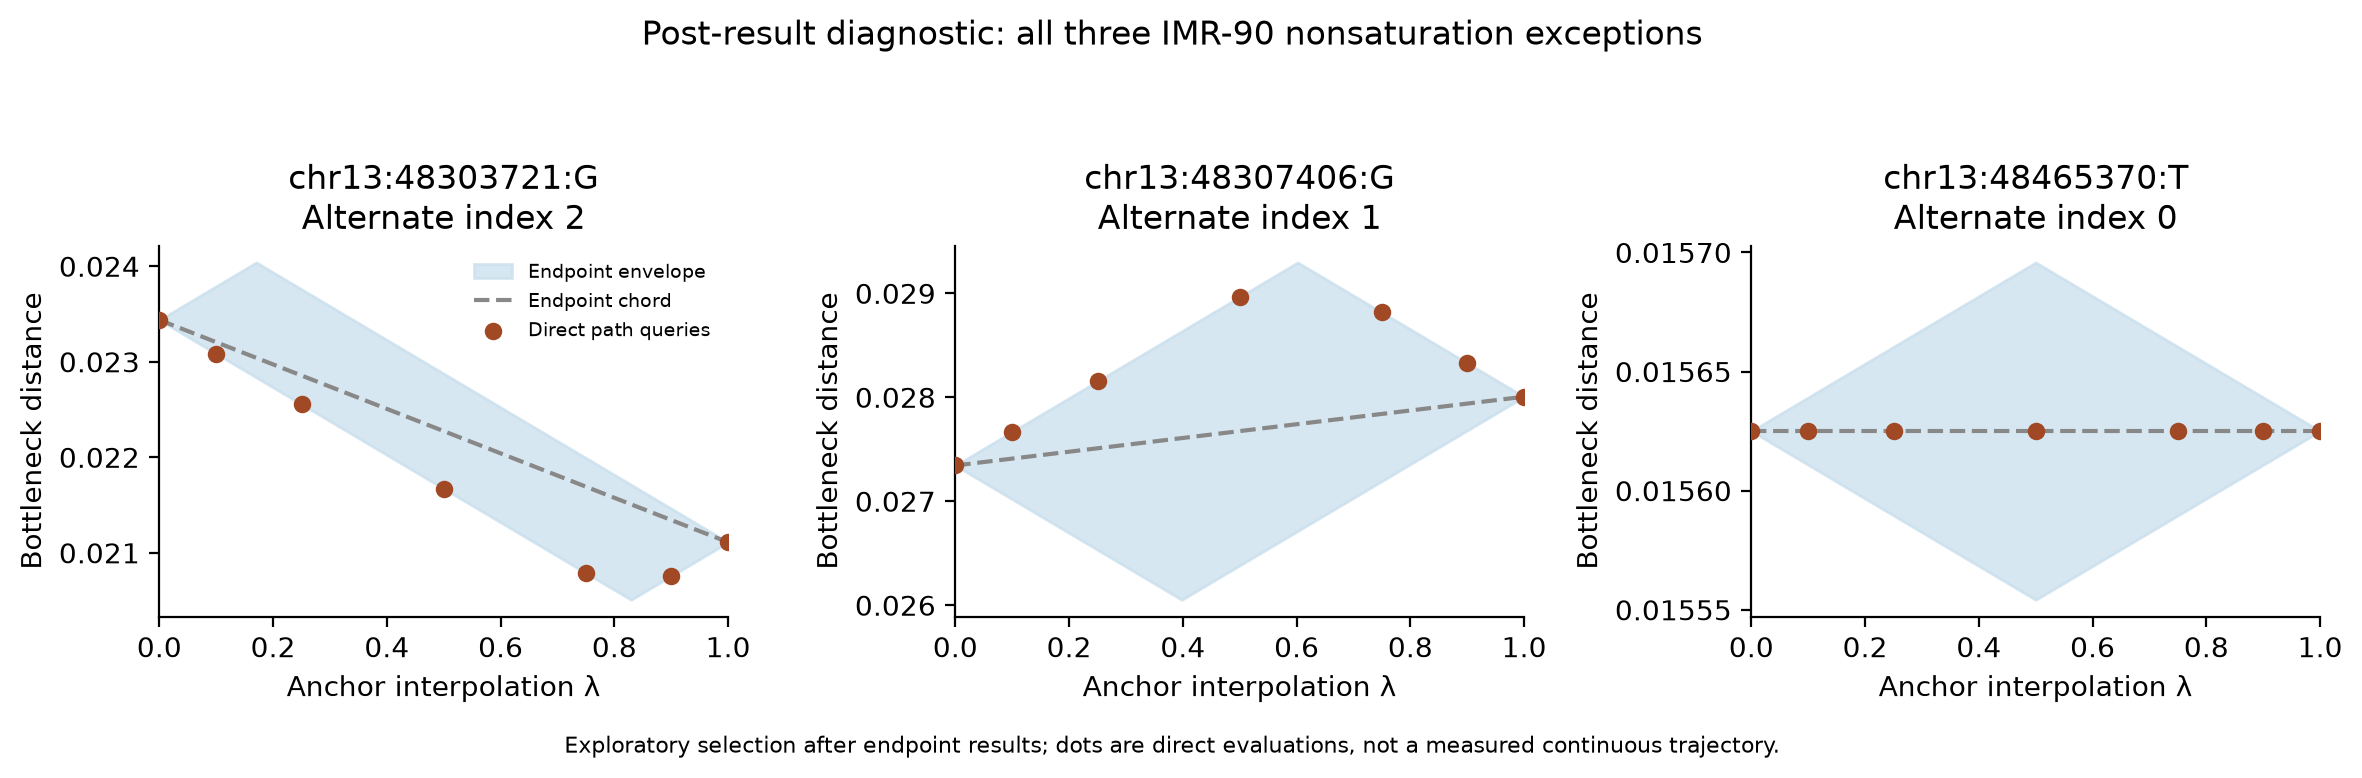
\includegraphics[keepaspectratio,alt={Exploratory direct path checks for all three exceptions}]{figures/figure_s4_exception_paths.png}}

\par\noindent\begin{minipage}{\linewidth}

\textbf{Figure S4.1.} Post-result exploratory calculations for all three
RB1 saturation exceptions. Points are direct matching computations at
the seven specified lambda values and do not certify intervening
behavior. Endpoint envelopes use their analytical kink vertices. Two
sampled paths change direction, while one is effectively flat. Dashed
chords are shown as a comparison, not an assumed interpolation. No exact
turning location or matching identity is inferred.

\end{minipage}\par

\end{document}
